\documentclass[9pt,twocolumn,twoside,]{pnas-new}

% Use the lineno option to display guide line numbers if required.
% Note that the use of elements such as single-column equations
% may affect the guide line number alignment.


\usepackage[T1]{fontenc}
\usepackage[utf8]{inputenc}

% tightlist command for lists without linebreak
\providecommand{\tightlist}{%
  \setlength{\itemsep}{0pt}\setlength{\parskip}{0pt}}




\templatetype{pnasresearcharticle}

\title{Réseau écologique des étudiants de Sherbrooke}

\author[]{}
\author[]{}
\author[]{}
\author[]{}



% Please give the surname of the lead author for the running footer
\leadauthor{}

% Please add here a significance statement to explain the relevance of your work
\significancestatement{}


\authorcontributions{}



\correspondingauthor{\textsuperscript{} }

% Keywords are not mandatory, but authors are strongly encouraged to provide them. If provided, please include two to five keywords, separated by the pipe symbol, e.g:


\begin{abstract}

\end{abstract}

\dates{This manuscript was compiled on \today}
\doi{\url{www.pnas.org/cgi/doi/10.1073/pnas.XXXXXXXXXX}}

\begin{document}

% Optional adjustment to line up main text (after abstract) of first page with line numbers, when using both lineno and twocolumn options.
% You should only change this length when you've finalised the article contents.
\verticaladjustment{-2pt}



\maketitle
\thispagestyle{firststyle}
\ifthenelse{\boolean{shortarticle}}{\ifthenelse{\boolean{singlecolumn}}{\abscontentformatted}{\abscontent}}{}

% If your first paragraph (i.e. with the \dropcap) contains a list environment (quote, quotation, theorem, definition, enumerate, itemize...), the line after the list may have some extra indentation. If this is the case, add \parshape=0 to the end of the list environment.

\acknow{}

\hypertarget{introduction}{%
\section{Introduction}\label{introduction}}

Texte ici

\hypertarget{ruxe9sultats}{%
\section{Résultats}\label{ruxe9sultats}}

\hypertarget{section-1}{%
\subsection{Section 1}\label{section-1}}

Texte ici

\hypertarget{section-2}{%
\subsection{Section 2}\label{section-2}}

Texte ici

\hypertarget{section-3}{%
\subsection{Section 3}\label{section-3}}

Texte ici

\hypertarget{muxe9thode}{%
\section{Méthode}\label{muxe9thode}}

\hypertarget{section-1-1}{%
\subsection{Section 1}\label{section-1-1}}

Texte ici

\hypertarget{section-2-1}{%
\subsection{Section 2}\label{section-2-1}}

Texte ici

\hypertarget{section-3-1}{%
\subsection{Section 3}\label{section-3-1}}

Texte ici

\hypertarget{discussion}{%
\section{Discussion}\label{discussion}}

\hypertarget{section-1-2}{%
\subsection{Section 1}\label{section-1-2}}

Texte ici

\hypertarget{section-2-2}{%
\subsection{Section 2}\label{section-2-2}}

Texte ici

\hypertarget{section-3-2}{%
\subsection{Section 3}\label{section-3-2}}

Texte ici

\hypertarget{conclusion}{%
\section{Conclusion}\label{conclusion}}

\hypertarget{bibliographie}{%
\section{Bibliographie}\label{bibliographie}}

References should be cited in numerical order as they appear in text;
this will be done automatically via bibtex, e.g. @belkin2002using and
@berard1994embedding {[}@coifman2005geometric{]}. All references,
including for the SI, should be included in the main manuscript file.
References appearing in both sections should not be duplicated. SI
references included in tables should be included with the main reference
section.

\hypertarget{figure-et-tableau}{%
\section{Figure et tableau}\label{figure-et-tableau}}

\begin{figure}
\centering
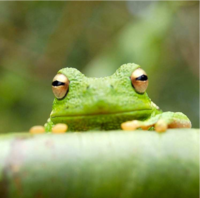
\includegraphics{frog.png}
\caption{Placeholder image of a frog with a long example caption to show
justification setting.{}}
\end{figure}

Figures and Tables should be labelled and referenced in the standard way
using the \texttt{\textbackslash{}label\{\}} and
\texttt{\textbackslash{}ref\{\}} commands.

Figure \[fig:frog\] shows an example of how to insert a column-wide
figure. To insert a figure wider than one column, please use the
\texttt{\textbackslash{}begin\{figure*\}...\textbackslash{}end\{figure*\}}
environment. Figures wider than one column should be sized to 11.4 cm or
17.8 cm wide.

\[\begin{aligned}
(x+y)^3&=(x+y)(x+y)^2\\
       &=(x+y)(x^2+2xy+y^2) \label{eqn:example} \\
       &=x^3+3x^2y+3xy^3+x^3. 
\end{aligned}\]



% Bibliography
% \bibliography{pnas-sample}

\end{document}
